\documentclass[a4paper, 12pt]{article}


\usepackage[czech]{babel}
\usepackage[utf8]{inputenc}
\usepackage[left=2cm, text={17cm, 24cm}, top=3cm]{geometry}
\usepackage{times}
\usepackage{verbatim}
\usepackage{enumitem}
\usepackage{graphicx}
\usepackage{amsthm, amsmath, amssymb}
\usepackage[unicode]{hyperref}
\usepackage{pdfpages}
\usepackage{pdflscape}
\usepackage{everypage}
\usepackage{fancyvrb}

\def\fillandplacepagenumber{%
 \par\pagestyle{empty}%
 \vbox to 0pt{\vss}\vfill
 \vbox to 0pt{\baselineskip0pt
   \hbox to\linewidth{\hss}%
   \baselineskip\footskip
   \hbox to\linewidth{%
     \hfil\thepage\hfil}\vss}}

\newcommand{\Lpagenumber}{\ifdim\textwidth=\linewidth\else\bgroup
  \dimendef\margin=0 %use \margin instead of \dimen0
  \ifodd\value{page}\margin=\oddsidemargin
  \else\margin=\evensidemargin
  \fi
  \raisebox{\dimexpr -\topmargin-\headheight-\headsep-0.5\linewidth}[0pt][0pt]{%
    \rlap{\hspace{\dimexpr \margin+\textheight+\footskip}%
    \llap{\rotatebox{90}{\thepage}}}}%
\egroup\fi}
\AddEverypageHook{\Lpagenumber}%


\begin{document}


% Titulní stránka %

	\begin{titlepage}
		\begin{center}
			
\includegraphics[width=0.77\linewidth]{FIT_logo.pdf} \\

			\vspace{\stretch{0.382}}

			\Huge{Projektová dokumentace} \\
			\LARGE{\textbf{Implementace překladače imperativního jazyka IFJ20}} \\
			\Large{Tým 75, varianta 1}
			
		\end{center}
        \begin{center}
	            \Large{Implementovaná rozšíření: \textbf{BASE}}
	            \vspace{\stretch{0.618}}
		\end{center}
		\begin{minipage}{0.4 \textwidth}
			{\Large \today}
		\end{minipage}
		\hfill
		\begin{minipage}[r]{0.6 \textwidth}
			\Large
			\begin{tabular}{l l l}
				\textbf{Michal Pyšík} & (xpysik00) & \quad 25\,\% \\
				Karel Jirgl & (xjirgl01) & \quad 25\,\% \\
				Václav Klem & (xklemv00) & \quad 25\,\% \\
				Thanh Quang Tran & (xtrant02) & \quad 25\,\% \\
			\end{tabular}
		\end{minipage}
	    
	\end{titlepage}

\tableofcontents

\newpage


\section{Spolupráce v týmu}
\subsection{Rozdělení práce v týmu}
Rozdělení práce probíhalo v době plánování. Nakonec jsme si všichni v různých částech implementace pomáhali, aby nebyl problém spojit všechny části předkladače v jeden funkční celek. Shodli jsme se na rovnoměrném rozdělení bodů, jelikož všichni členové týmu spolu aktivně komunikovali, pomáhali si a nebyly žádné významné neshody. 

\subsubsection*{Michal Pyšík (xpysik00)}
Implementace lexikálního analyzátoru a ustanovení typů tokenů

\subsubsection*{Karel Jirgl (xjirgl01)}
Gramatika, Syntaktická a sémantická analýza, implementace tabulky symbolů, LL tabulky, precedenční~syntaktické analýzy

\subsubsection*{Václav Klem (xklemv00) }
Generátor cílového kódu

\subsubsection*{Thanh Quang Tran (xtrant02)}
Gramatika, LL tabulka, tabulka precedenční syntaktické analýzy 

\subsubsection*{Společná práce}
Dokumentace, obecná struktura cílového programu

\subsection{Způsob práce v týmu}
Komunikace probíhala především prostřednictvím Discord serveru vytvořeného přímo pro tento projekt. Konaly se pravidelné porady a všichni členové týmu byli většinou k dispozici, pokud se vyskytl nějaký problém nebo bylo potřeba se dohodnout na konkrétních detailech implementace. Díky úspěšné komunikaci a vzájemnému porozumnění kódu mezi kolegy nebyl problém spojit jednotlivé části tak, aby spolu byly vzájemně kompatibilní. Pro správu zdrojových souborů jsme používali verzovací systém Git, většina práce se odehrávala pouze v hlavní větvi, jelikož v konkrétním souboru prováděla změny většinou jen jedna osoba najednou.

\newpage

\section{Lexikální analýza}
První částí překladače je lexikální analyzátor (scanner). Nejdůležitější funkcí je zde \linebreak \verb|scannerGetToken|, což je vlastně implementace deterministického konečného automatu, který čte jednotlivé znaky ze standartního vstupu, dokud nedojde do koncového stavu (návratová hodnota 0), nebo nenarazí na lexikální chybu (návratová hodnota 1). To je zajištěné pomocí přepínače \verb|switch| umístěného v nekonečném \verb|while| cyklu, kde každý \verb|case| reprezentuje právě jeden stav automatu, a při každém opakování cyklu je čten právě jeden znak ze vstupu.
\newline
\newline
Funkce má jediný parametr, a to ukazatel na předem alokovaný prvek typu \verb|Token|, jehož typ (a případně atribut) se nastaví podle přečtených hodnot a dosaženého koncového stavu. Mezi typy tokenů bez atributů patří například relační operátory, aritmetické operátory, přiřazení, klíčová slova, odřádkování (\verb|EOL|), konec souboru (\verb|EOF|), závorky a další povolené znaky.
\newline
\newline
Typy tokenů s atributy jsou pouze identifikátor, celé číslo, desetinné číslo a řetězec. Atribut tokenu je typu \verb|union|, v případě identifikátoru nebo řetězce se tedy využívá pouze atribut \verb|string|, u celého čísla \verb|integer| a u desetinného čísla \verb|real|. Když je zřejmé že načítáme nějaký z těchto 4 typů tak se přečtené znaky nejprve ukládají do bufferu (globální pole), a ve chvíli kdy je dosaženo koncového stavu, se do následující pozice v bufferu vloží nulový znak. Obsah bufferu až po tento znak je poté převeden na celé/desetinné číslo, nebo zkopírován do nově alokovaného stringu (jehož velikost pro alokaci je index pozice prvního nulového znaku v bufferu + 1). Tento postup je velice praktický, protože i když se obsah bufferu nemaže ale pouze přepisuje, cokoli za prvním nulovým znakem je ignorováno, například pozůstatky nějakého delšího dříve načteného řetězce. V případě ID se ještě zavolá funkce \verb|keywordCheck|, která kontroluje zda se nejedná o klíčové slovo, v takovém případě uvolní alokovaný \verb|string| a nastaví odpovídající typ tokenu.
\newline
\newline
Všechny načtené tokeny se ukládají do obousměrně vázaného lineárního seznamu \verb|tokenList|, který je předáván dalším částem překladače. Z pracujících se seznamem stojí za zmínku \linebreak\verb|ScannerGetTokenList|, která plní seznam tokeny (voláním dříve popsané funkce), dokud nenarazí na token typu \verb|EOF|, nebo volaná funkce nenahlásí lexikální chybu. 

\subsection{Graf konečného stavového automatu lexikálního analýzátoru}
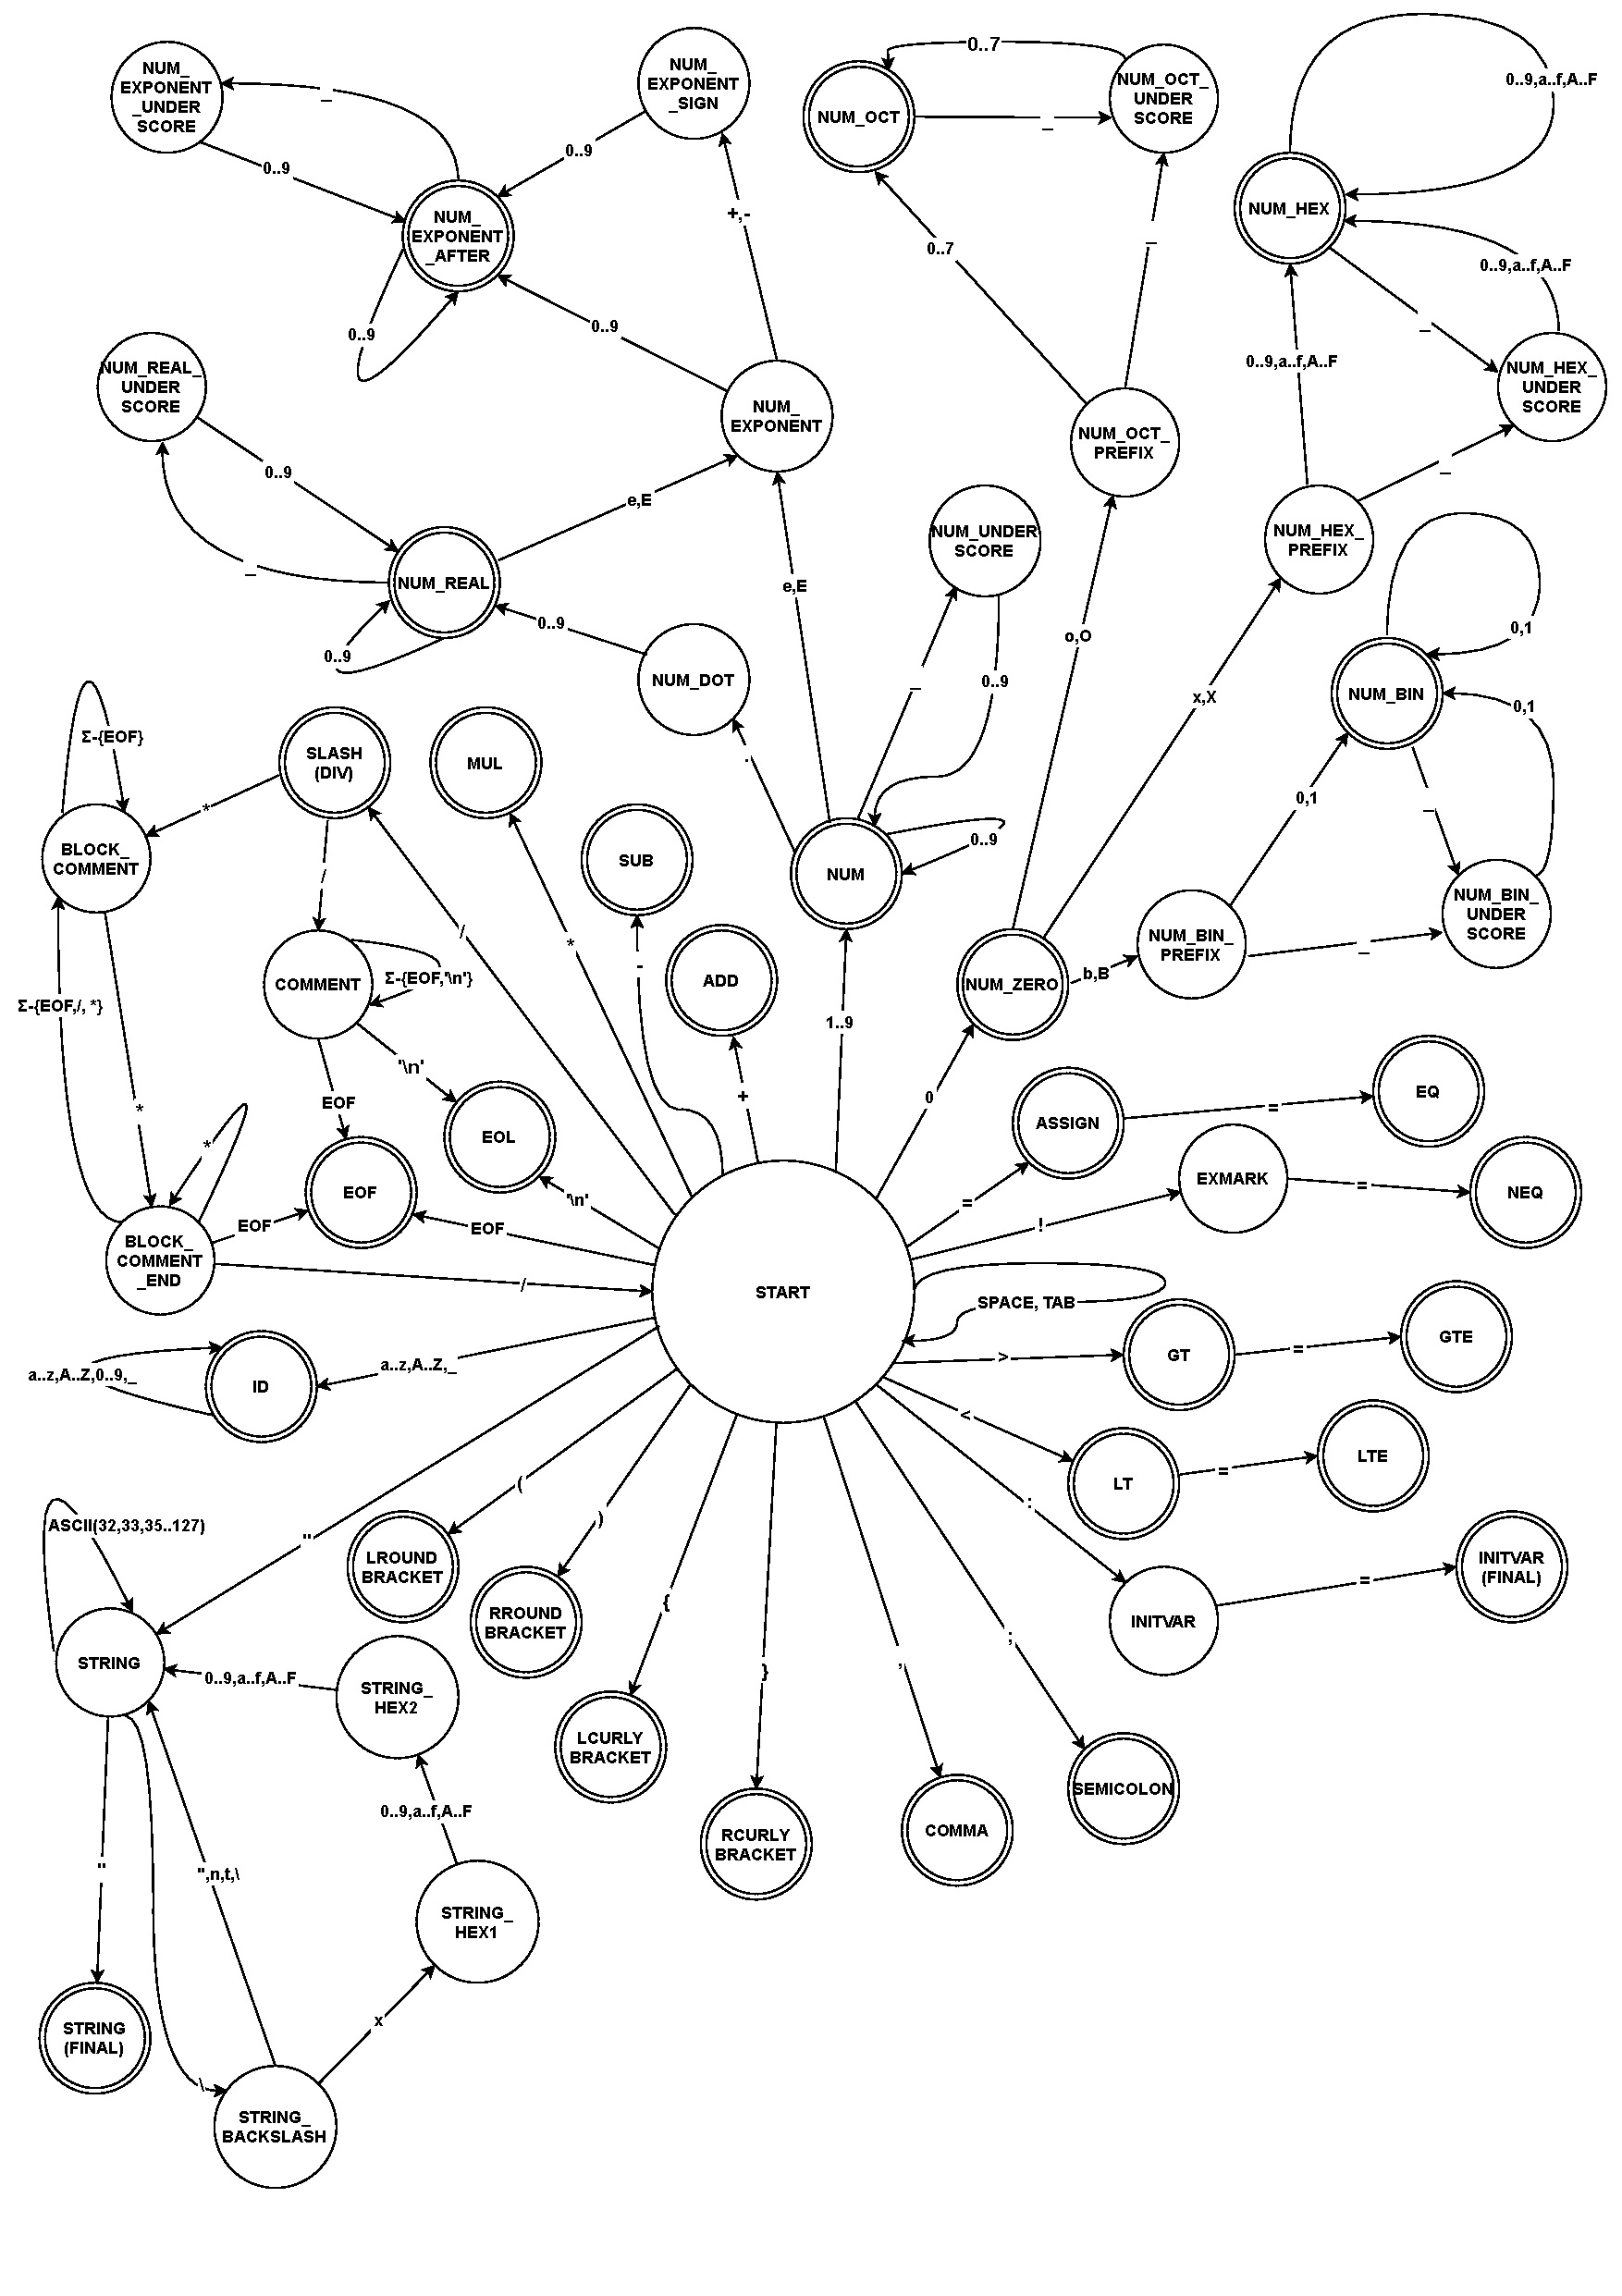
\includegraphics[height=24cm,keepaspectratio]{Scanner_FSM_Graph.pdf}

\section{Syntaktická a sémantická analýza (parser)}
Celá syntaktická a sémantická analýza se odehrává v souboru parser.c a konkrétně se spouští funkcí parserAnalyze.

V našem projektu je funkce parserAnalyze přímo volána z hlavní funkce main se vstupním parametrem tokenList, který obsahuje kompletní seznam tokenů načtený skenerem, který je implementován jako dynamický obousměrný lineární seznam. První akcí této funkce je vytvoření globální tabulky symbolů.

Proces parseru se skládá ze dvou hlavních funkcí:

parserPreRun – zde dojde k naplnění globální tabulky symbolů uživatelskými a vestavěnými funkcemi, vytvoření jejich lokálních tabulek symbolů a uložení důležitých informací o nich (počet vstupních a výstupních parametrů a datové typy parametrů).

parserRunPredictiveSyntaxAnalysis – spuštění samotného procesu syntaktické a sémantické analýzy.

\subsection{Implementace funkce \protect\Verb|parserPreRun|}
Hned na začátku funkce dojde k naplnění globální tabulky symbolů vestavěnými funkcemi voláním funkce \verb|parserSymTableInitBuiltIn|.

Dále se v cyklu prochází celý tokenList, kde se očekává token \verb|TOKEN_KEYWORD_FUNC| následovaný tokenem \verb|TOKEN_ID|, což značí začátek definice funkce. V globální tabulce symbolů se zkontroluje, že se nejedná o redefinici funkce a vloží se do ní záznam nové funkce, který bude obsahovat seznam typů vstupních parametrů a seznam typů výstupních parametrů funkce. Do záznamu se také přidá nová lokální tabulka symbolů, kam se přidají proměnné vstupních parametrů a proměnná blackhole (\verb|‚_‘|).

Nakonec se kontroluje výskyt prologu (token \verb|TOKEN_KEYWORD_PACKAGE|), výskyt hlavní funkce main, a že funkce main nemá žádné vstupní ani výstupní parametry.

\subsection{Proces analýzy - funkce \protect\Verb|parserRunPredictiveSyntaxAnalysis|}
Na začátku funkce parserRunPredictiveSyntaxAnalysis dojde k nastavení ukazatele aktivního prvku tokenList na první prvek a spouští se analýza kódu.

\subsubsection{Syntaktická analýza celého kódu}
Pro syntaktickou analýzu kódu je použita Prediktivní syntaktická analýza. Na syntaktický zásobník je na počátku vložen neterminální stav \verb|NONTERM_PROGRAM| a zároveň s \verb|tokenList| je zásobník procházen v cyklu se třemi podmínkami:

\begin{enumerate}
    \item Pokud je na zásobníku terminál \verb|TERM_EOF|, zkontroluje se i aktuální čtený token, zda je roven tokenu \verb|TOKEN_EOF|. V případě platnosti je analýza ukončena s pozitivním výsledkem – syntaxe i sémantika je správně. V případě, že na zásobníku je terminál \verb|TERM_EOF|, ale aktuální token není \verb|TOKEN_EOF|, je vrácena chyba špatného tokenu na vstupní pásce.
    \newpage
    \item Jestliže se na zásobníku nachází neterminál, nalezne se podle aktuálního tokenu na vstupu
    v LL-tabulce číslo pravidla pro jeho rozklad. Pokud nebylo pravidlo nalezeno, došlo k syntaktické chybě. Jinak se ze zásobníku odstraní daný neterminál a nahradí se pravou stranou pravidla ze seznamu pravidel podle LL-tabulky. LL-tabulka i seznam pravidel je uložen v souboru common.h. Číslo pravidla je uloženo do zásobník s posloupností čísel pravidel pravého a levého rozboru.
    \item Při terminálu na zásobníku jsou tři možnosti. Pokud terminálem je \verb|TERM_PSEUDO_EPSILON|, pouze se zahodí ze zásobníku. Při neterminálu \verb|TERM_EXPRESSION| se uloží do seznamu všechny tokeny výrazu a spustí se precedenční analýza výrazu. Jestliže terminál na zásobníku je roven tokenu ze vstupu, spustí se Sémantická analýza, zahodí se první neterminál na zásobníku a posune se ukazatel na vstupním seznamu tokenů na další token.
\end{enumerate}
\subsubsection{Syntaktická analýza výrazů}
Syntaxe výrazů je kontrolována pomocí precedenční analýzy a precedenční tabulky (uložena v souboru common.h). Na začátku je na precedenční zásobník vložen pseudoterminál \linebreak \verb|TERM_PSEUDO_DOLLAR|, sloužící jako počáteční a ukončovací symbol. V cyklu \verb|while| z precedenční tabulky získáme jednu ze tří operaci, která se má provést. Získáme ji z aktuálního tokenu na vstupu a nejvýše uloženého terminálu na precedenčním zásobníku. Pokud v precedenční tabulce není nalezena žádná operace, je vrácena syntaktická chyba. Před provedením některé ze tří operací se zkontroluje, že nejvýše uložený terminál na precedenčním zásobníku se nerovná \verb|TERM_PSEUDO_DOLLAR| a aktuální načtený token se nerovná \verb|TERM_PSEUDO_DOLLAR|. V opačném případě je voláno paralelně běžící Generování kódu výrazu a Precedenční analýza ukončena s kladným výsledkem.
\begin{enumerate}
    \item Pokud je aktuální operace „$=$“ (rovná se), zavolá se paralelně běžící Sémantická analýza, na precedenční a sémantický zásobník se přidá aktuálně čtený token a nakonec se posune čtecí hlava tokenů na další token.
    \item Při operaci „$<$“ (menší než) se provede to stejné, co při operaci „$=$“, ale k tomu navíc se přidá na precedenční zásobník terminál \verb|TERM_PSEUDO_HANDLE|, který slouží pro označení začátku syntaktického pravidla pro další syntaktickou kontrolu.
    \item Nastane-li operace „$>$“ (větší než), zavolá se na začátku paralelně běžící Generování kódu.  Poté se najde v LL-tabulce pravidlo, které je rovno posloupnosti terminálů a neterminálů na precedenčním zásobníku od terminálu \verb|TERM_PSEUDO_HANDLE| po vrchol zásobníku a nahradí se za levou stranu nalezeného pravidla. Pokud není pravidlo nalezeno, jedná se o syntaktickou chybu. Také je uloženo číslo pravidla do zásobník s posloupností čísel pravidel pravého a levého rozboru.
\end{enumerate}

\newpage

%%%%%%%%%%%%%%%% semantics analysis %%%%%%%%%%%%%%%%%%%%%%%%%%%%%%%%%%
\subsection{Sémantická analýza}
Sémantická analýza běží paralelně se syntaktickou analýzou a její funkce parserSemanticAnalysis je volána pro každý přečtený token zvlášť. Sémantické chyby jsou kontrolovány pomocí podmínek, které očekávají určitý token nebo posloupnost tokenů anebo také stavy uložené v pomocných proměnných. Tyto podmínky můžeme rozdělit na globální a řádkové kontroly.
\begin{itemize}
    \item \textbf{DEFINICE FUNKCE} – zkontroluje se, že je funkce definována v globální tabulce symbolů a její lokální tabulka symbolů se přidá na zásobník tabulek symbolů
    \item \textbf{VSTUP DO NOVÉHO ROZSAHU PLATNOSTI} – při levé složené závorce '\{' nebo klíčovém slově for se zvýší úroveň zanoření a vytvoří se nová tabulka symbolů, která se vloží do zásobníku tabulek symbolů
    \item \textbf{UKONČENÍ ROZSAHU PLATNOSTI} – při pravé složené závorce '\}' jednou nebo dvakrát při ukončení cyklu for se sníží úroveň zanoření a odstraní vrchní tabulka symbolů ze zásobníku tabulek symbolů
    \item \textbf{KONEC DEFINICE FUNKCE} - při pravé složené závorce '\}' a pouze s poslední tabulkou symbolů (lokální tabulka symbolů funkce) se z kontroluje existence klíčového slova return
    \item \textbf{RETURN NENALEZEN} - při levé složené závorce '\{' nastavíme returnExists na false
    \item \textbf{RETURN NALEZEN} - při klíčovém slově return nastavíme returnExists na true
\end{itemize}


\begin{landscape}
\pagestyle{empty}
\begin{figure}[h]
\subsection{LL tabulka}
\hspace*{-3.6cm}\vspace*{+1cm}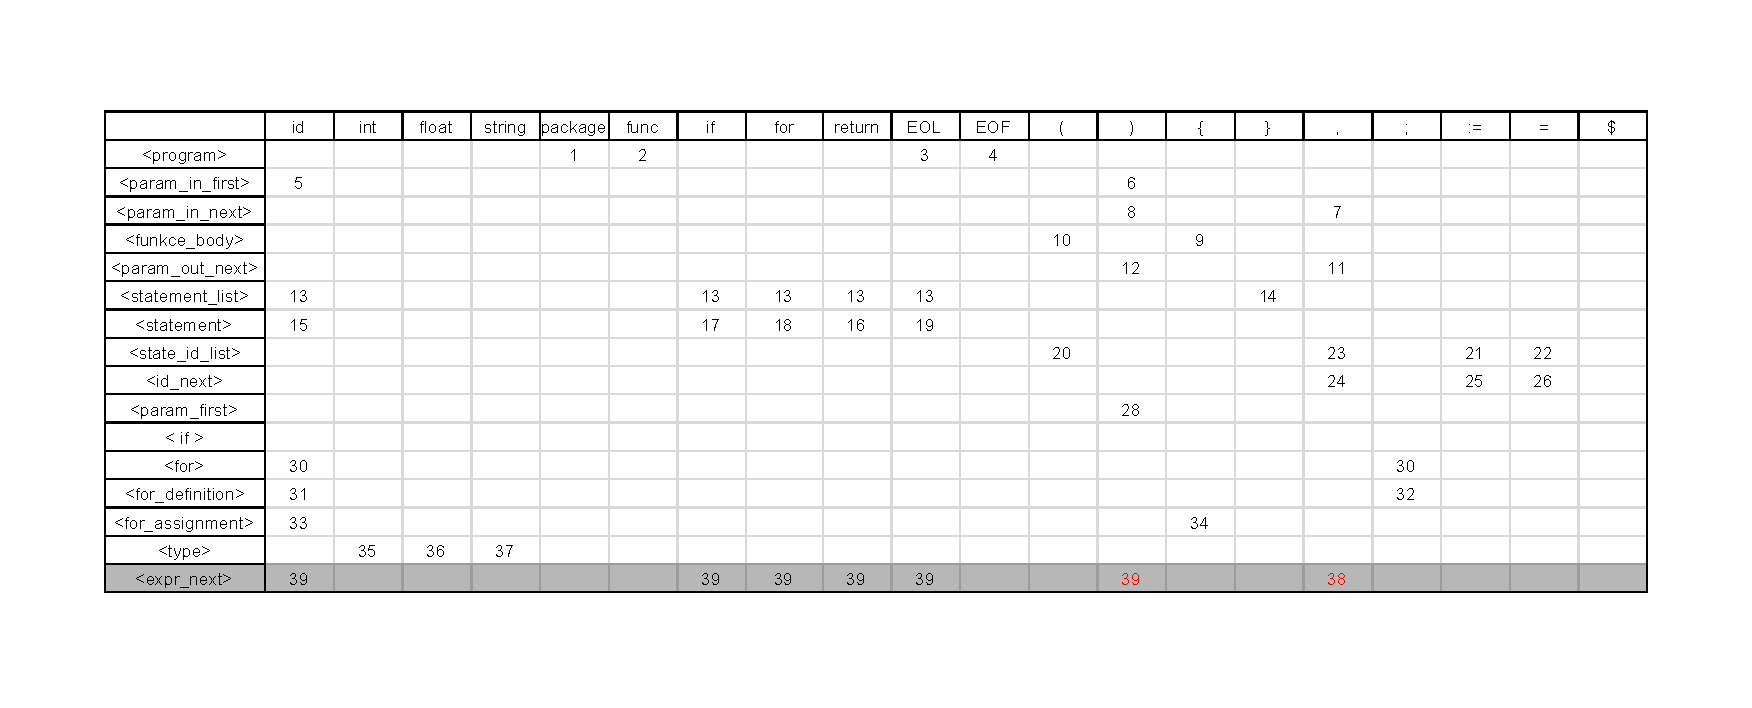
\includegraphics[width=1.85\textwidth,keepaspectratio]{LL_table.pdf}
%\fillandplacepagenumber
\end{figure}
\end{landscape}

\begin{landscape}
\pagestyle{empty}
\begin{figure}[h]
\subsection{Precedenční tabulka}
\hspace*{-3.6cm}\vspace*{+1cm}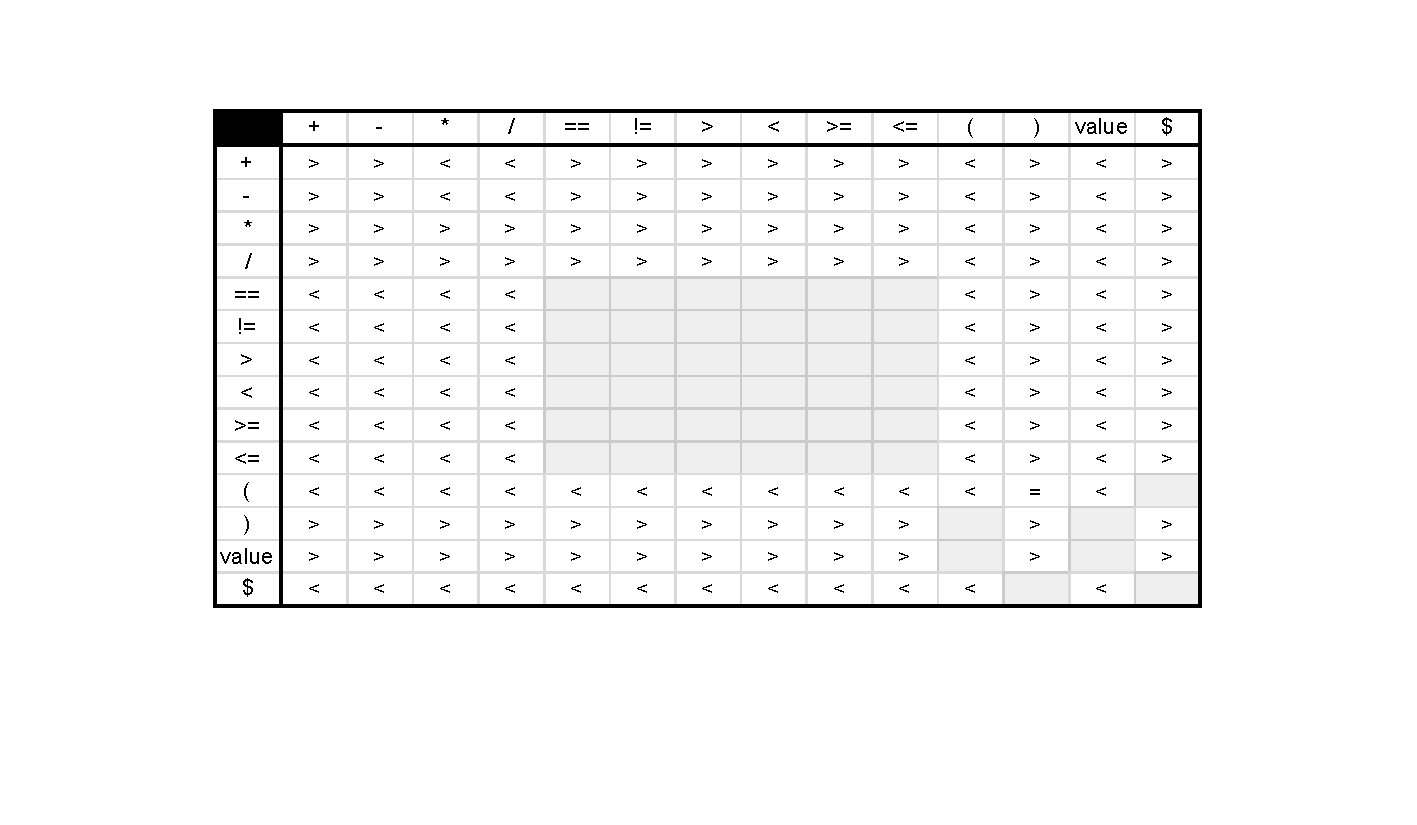
\includegraphics[width=1.85\textwidth,keepaspectratio]{Precedence_table.pdf}
%\fillandplacepagenumber
\end{figure}
\end{landscape}

\newpage

\subsection{LL -- gramatika}

		\begin{enumerate}[noitemsep]
		\footnotesize{
            \item \verb|<program> -> package id EOL <program>| 
            \item \verb|<program> -> func id ( <param_in_first> ) <func_body> <program>|
            \item \verb|<program> -> EOL <program>|
            \item \verb|<program> -> EOF |
            
            \item \verb|<param_in_first> -> id <type> <param_in_next> |
            \item \verb|<param_in_first> ->| $\varepsilon$
            \item \verb|<param_in_next> -> , id <type> <param_in_next>|
            \item \verb|<param_in_next> -> | $\varepsilon$
            
            \item \verb|<func_body> -> { EOL <statements> }|
            \item \verb|<func_body> -> ( <type> <param_out_next> ) { EOL <statements> } |
            
            \item \verb|<param_out_next> -> , <type> <param_out_next> |
            \item \verb|<param_out_next> ->| $\varepsilon$
            
            \item \verb|<type> -> int|
            \item \verb|<type> -> float| 
            \item \verb|<type> -> string|
            
            \item \verb|<statements> -> id <statement_id> EOL <statements>|
            \item \verb|<statements> -> return EXPRESSION <expr_next> EOL <statements>|
            \item \verb|<statements> -> if EXPRESSION { EOL <statements> }|\newline \verb|                else { EOL <statements> } EOL <statements>|
            \item \verb|<statements> -> for <for_definition> ; EXPRESSION ; <for_assignment>|\newline \verb|                { EOL <statements> } EOL <statements>|
            \item \verb|<statements> -> EOL <statements>|
            \item \verb|<statements> ->| $\varepsilon$
            
            \item \verb|<statement_id> -> ( <arg_first> )|
            \item \verb|<statement_id> -> := <id_expression>|
            \item \verb|<statement_id> -> = <id_expression>|
            \item \verb|<statement_id> -> , id <id_next>|
            
            \item \verb|<id_next> -> , id <id_next>|
            \item \verb|<id_next> -> = <ids_expression>|
            
            \item \verb|<for_definition> -> id := <ids_expression>|
            \item \verb|<for_definition> -> | $\varepsilon$
            
            \item \verb|<for_assignment> -> id := <for_assign_id>|
            \item \verb|<for_assignment> -> | $\varepsilon$
            \item \verb|<for_assign_id> -> , id <for_assign_id>|
            \item \verb|<for_assign_id> -> = <ids_expression>|
            
            \item \verb|<id_expression> -> id ( <arg_first> )|
            \item \verb|<id_expression> -> <expr>|
            
            \item \verb|<ids_expression> -> id ( <arg_first> )|
            \item \verb|<ids_expression> -> <expr> <expr_next>|
            
            \item \verb|<expr_next> -> , <expr> <expr_next>|
            \item \verb|<expr_next> ->| $\varepsilon$
        
            \item \verb|<arg> -> INT|
            \item \verb|<arg_first> -> INT <arg_next>|
            \item \verb|<arg_first> -> FLOAT <arg_next>|
            \item \verb|<arg_first> -> STRING <arg_next>|
            \item \verb|<arg_first> -> id <arg_next>|
            \item \verb|<arg_first> ->| $\varepsilon$
           
            \item \verb|<arg_next> -> , <arg> <arg_next>|
            \item \verb|<arg_next> ->| $\varepsilon$
            \item \verb|<arg> -> FLOAT|
            \item \verb|<arg> -> STRING|
            \item \verb|<arg> -> id| 
            }
            
            
        \end{enumerate} 

\newpage

\section{Tabulka symbolů}

\section{Generace mezikódu IFJcode20}
Generování cílového kódu IFJcode20 probíhá vždy po každém dokončení jedné iterace syntaktické a sémantické analýzy. Parser generátoru sekvenčně předává pravidla LL tabulky pravého a levého rozboru a sémantický stack, který obsahuje tokeny pro generování aritmetických a logických výrazů. Scanner poskytuje double-linked list tokenů z lexikálního analyzátoru.
\newline
\newline
Hlavní funkcí je \verb|generatorGenerateCode|, která tiskne instrukce prostřednictvím přepínače \verb|switch| a instrukce aritmetických a logických operací prostřednictvím podmíněného cyklu \verb|while| za pomocí sémantického zásobníku předávaného parserem.\\
\newline
Ke generování podmíněného příkazu \verb|if| / \verb|else| a cyklů \verb|for| je kvůli správnému výpisu návěští \verb|LABEL| použit zásobník na ukládání celočíselných hodnot, které reprezentují jednotlivé ID daných klíčových slov. K uchování informací o momentálním kontextu v kódu IFJ20 slouží \verb|static| proměnné.\\
\newline

\section{Hlavní funkce main}
Funkce main předá errorHandle nastavený na stderr a rozjede překladač a vyplivne cílový kód. 
\end{document}